\chapter{Virología}\label{ch:b3:virology}

Hay en la Tierra unas $10^{31}$ partículas víricas, diez por cada célula,
y en el mar matan cada día a una quinta parte de todas las bacterias. Un
\omterm{def:b3:virology:virus}{virus} no es una célula: no tiene metabolismo, ni ribosomas, ni manera
alguna de fabricar nada por sí mismo. Es un genoma --- tan corto como dos
genes, tan largo como dos mil --- envuelto en una cubierta proteica, que
entra en una célula y vuelve la maquinaria de esta a fabricar copias de
sí mismo. La gripe de 1918 mató a cincuenta millones de personas; la
viruela, que mató a trescientos millones solo en el siglo~XX, se erradicó
en 1980 con una \omterm{def:b3:virology:drugs}{vacuna} ensayada por primera vez en 1796; y un coronavirus
que pasó al ser humano en 2019 tuvo su genoma secuenciado en cuestión de
semanas, una \omterm{def:b3:virology:drugs}{vacuna} diseñada pocos días después y fármacos contra su
proteasa en menos de dos años. Este capítulo trata de qué son los \omterm{def:b3:virology:virus}{virus} y
de cómo se clasifican por la química de sus genomas, de cómo se
multiplican, de la cinética de una infección dentro de un hospedador ---
que un par de ecuaciones diferenciales describe lo bastante bien como
para haber cambiado el tratamiento del sida ---, de su evolución y de
cómo se combaten.

\section{Qué es un virus}

\begin{definition}[Virus]\label{def:b3:virology:virus}
\index{virus}\index{cápside}\index{envoltura}\index{virión}\index{clasificación de Baltimore}
Un \emph{virus} es un parásito intracelular obligado que consta de un
genoma de ácido nucleico --- ADN o ARN, de hebra sencilla o doble, lineal
o circular, en una molécula o en varias --- empaquetado en una
\emph{cápside} proteica y, en muchos casos, envuelto en una
\emph{envoltura} tomada de una membrana del hospedador y tachonada de
glicoproteínas víricas. La partícula infecciosa completa es el
\emph{virión}, de \qtyrange{20}{300}{nm} en la mayoría (unos pocos virus
gigantes llegan al micrómetro). Las cápsides se construyen con muchas
copias de una o de unas pocas proteínas dispuestas con simetría
helicoidal (una varilla, como en el virus del mosaico del tabaco) o
icosaédrica (una cubierta de $60T$ subunidades, con
$T = 1, 3, 4, 7,\dots$). La \emph{clasificación de Baltimore} agrupa los
virus por la ruta que va del genoma al ARN mensajero: I, ADN de doble
hebra (herpes, viruela, adenovirus, la mayoría de los fagos); II, ADN de
hebra sencilla (parvovirus); III, ARN de doble hebra (rotavirus); IV, ARN
de hebra positiva, que es él mismo un mensajero (polio, hepatitis C, los
coronavirus); V, ARN de hebra negativa, complementario del mensajero
(gripe, sarampión, rabia, Ébola); VI, ARN retrotranscrito a ADN (los
retrovirus, el VIH); VII, ADN que se replica a través de un intermediario
de ARN (hepatitis B). Todas las clases salvo la I han de traer o
codificar una enzima que la célula no tiene --- una ARN-polimerasa
dependiente de ARN, una transcriptasa inversa --- y esas enzimas son la
diana de casi todos los \omterm{def:b3:virology:drugs}{antivíricos}.
\end{definition}

\begin{proof}[Evidencia]
Ivanovski (1892) y Beijerinck (1898) mostraron que la enfermedad del
mosaico del tabaco se transmitía por savia pasada a través de filtros que
retenían todas las bacterias --- un \emph{contagium vivum fluidum}, un
fluido infeccioso vivo. Stanley (1935) cristalizó el agente, el \omterm{def:b3:virology:virus}{virus} del
mosaico del tabaco, y mostró que era proteína con (como hallaron Bawden y
Pirie) un \qty{5}{\%} de ARN. Hershey y Chase (1952) marcaron la proteína
de un bacteriófago con $^{35}$S y su ADN con $^{32}$P, lo dejaron
infectar \emph{E.~coli}, arrancaron en una batidora las cubiertas vacías
y encontraron el $^{32}$P dentro de las células y el $^{35}$S fuera: el
ADN entra y la proteína se queda, de modo que el ADN lleva las
instrucciones. Fraenkel-Conrat (1955) desmontó el \omterm{def:b3:virology:virus}{virus} del mosaico del
tabaco en proteína y ARN y volvió a montar partículas infecciosas con el
ARN de una cepa y la proteína de otra; la descendencia era de la cepa del
ARN.
\end{proof}

\begin{proposition}[Economía genética: por qué las cápsides son simétricas]\label{prop:b3:virology:economy}
\index{economía genética}
Una \omterm{def:b3:virology:virus}{cápside} ha de encerrar el genoma que la codifica. Una proteína de
masa $m$ necesita unos $m/\qty{110}{Da}$ codones, es decir, $3m/110$
nucleótidos, un tramo de ARN que pesa alrededor de
$3m/110\times\qty{330}{Da} = 9m$: toda proteína la codifica un ácido
nucleico nueve veces más pesado que ella. Una cubierta hecha de una
\emph{sola} molécula de proteína que encerrara un genoma tendría que
encerrar un genoma nueve veces su propia masa solo para codificarse a sí
misma, y una cubierta no puede contener nueve veces su propia masa de
ácido nucleico a densidad biológica. La salida, vista por Crick y Watson
(1956), es construir la cubierta con muchas copias de una proteína
pequeña: el \omterm{def:b3:virology:virus}{virus} del mosaico del tabaco codifica una proteína de
cubierta de \qty{17.5}{kDa} en \qty{480}{nt} de su genoma de
\qty{6400}{nt} y usa $2130$ copias de ella. Unas subunidades idénticas
que se empaquetan de forma idéntica han de disponerse simétricamente, de
modo que las \omterm{def:b3:virology:virus}{cápsides} víricas son hélices o icosaedros, y la misma
economía les da la capacidad de autoensamblarse, ya que cada subunidad
solo necesita reconocer a sus vecinas.
\end{proposition}
\begin{proof}
La razón de masas se sigue de que un codón son tres nucleótidos de unos
\qty{330}{Da} cada uno y un residuo unos \qty{110}{Da}: $3\times 330/110 =
9$. Una \omterm{def:b3:virology:virus}{cápside} de una sola proteína de \qty{40}{MDa} encerraría
\qty{360}{MDa} de ácido nucleico, una esfera de unos \qty{50}{nm} de
radio a densidad de ácido nucleico, mientras que la propia proteína daría
una cubierta de unos \qty{2}{nm} de espesor y el mismo radio ---
geométricamente posible, pero un solo polipéptido de $360\,000$ residuos
que se pliegue correctamente no lo es, y una sola mutación lo destruiría.
Con $n$ subunidades idénticas el coste de codificación cae por $n$
mientras el volumen encerrado no cambia.
\end{proof}

\begin{omfigure}
\begin{tikzpicture}[every node/.style={font=\scriptsize}, >=stealth]
  \node[draw, thick, rounded corners, fill=omMeth!30, minimum width=2.4cm] (mrna) at (0,0) {ARNm $\to$ proteína};
  \node[draw, thick, rounded corners, fill=omDef!20, align=center] (I) at (-5.8,3.6) {I: ADNbc\\herpes, viruela, fago T4};
  \node[draw, thick, rounded corners, fill=omDef!20, align=center] (II) at (-2.0,3.6) {II: ADNhs\\parvovirus};
  \node[draw, thick, rounded corners, fill=omThm!20, align=center] (III) at (2.0,3.6) {III: ARNbc\\rotavirus};
  \node[draw, thick, rounded corners, fill=omThm!20, align=center] (IV) at (5.8,3.6) {IV: ARN (+)\\polio, hepatitis C,\\coronavirus};
  \node[draw, thick, rounded corners, fill=omThm!20, align=center] (V) at (-5.6,-3.4) {V: ARN ($-$)\\gripe, sarampión,\\rabia, Ébola};
  \node[draw, thick, rounded corners, fill=omProp!30, align=center] (VI) at (0,-3.4) {VI: ARN $\to$ ADN\\retrovirus (VIH)};
  \node[draw, thick, rounded corners, fill=omProp!30, align=center] (VII) at (5.6,-3.4) {VII: ADN vía ARN\\hepatitis B};
  \node[below, font=\tiny, align=center, gray!50!black] at (-5.8,2.9) {ARN-polimerasa del hospedador};
  \node[below, font=\tiny, align=center, gray!50!black] at (-2.0,3.05) {se fabrica la segunda hebra\\y luego se transcribe};
  \node[below, font=\tiny, align=center, gray!50!black] at (2.0,3.05) {ARN-polimerasa vírica\\en la partícula};
  \node[below, font=\tiny, align=center, gray!50!black] at (5.8,2.75) {el genoma es el ARNm};
  \node[above, font=\tiny, align=center, gray!50!black] at (-5.6,-2.55) {la polimerasa vírica lo copia};
  \node[above, font=\tiny, align=center, gray!50!black] at (0,-2.85) {transcriptasa inversa, integración\\y luego polimerasa del hospedador};
  \node[above, font=\tiny, align=center, gray!50!black] at (5.6,-2.85) {transcripción del ADN};
  \foreach \c in {I,II,III,IV,V,VI,VII} \draw[->, thick] (\c) -- (mrna);
\end{tikzpicture}

{\small Las siete clases de Baltimore, ordenadas por la ruta que va del
genoma al ARN mensajero. Todas las clases salvo la I necesitan una enzima
que la célula hospedadora no aporta --- la diana natural de un \omterm{def:b3:virology:drugs}{antivírico}.}
\end{omfigure}

\begin{omfigure}
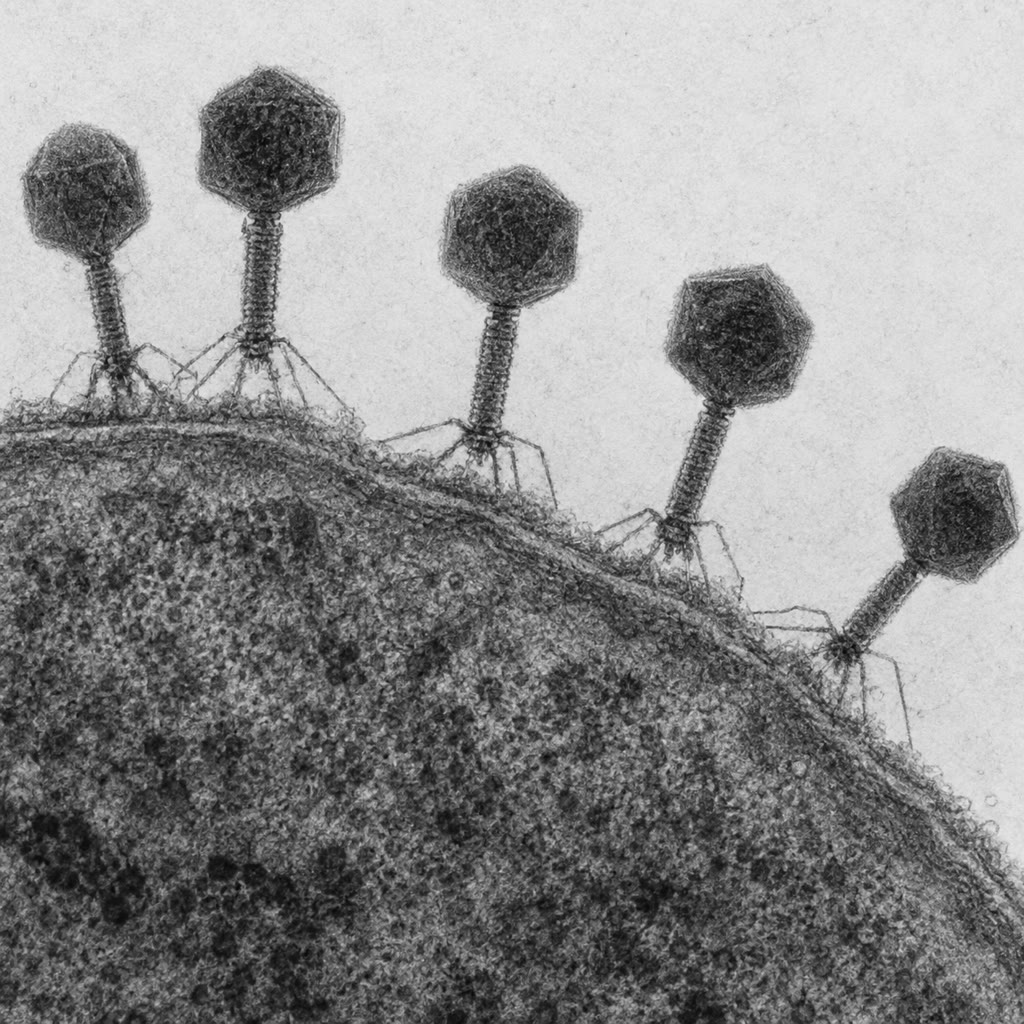
\includegraphics[width=0.36\linewidth]{images/book5/ai/b5-13-phage-tem.jpg}\hspace{0.04\linewidth}
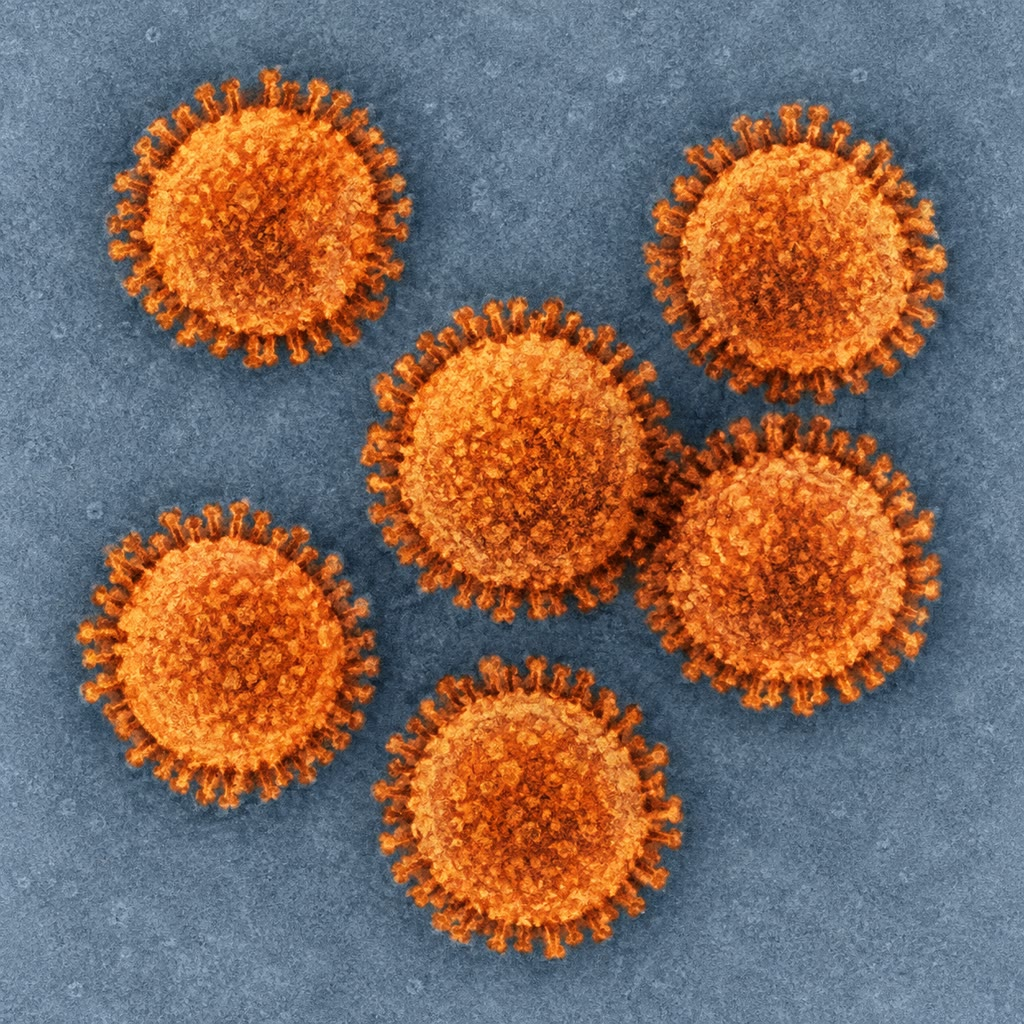
\includegraphics[width=0.36\linewidth]{images/book5/ai/b5-13-influenza-virions.jpg}

{\small Izquierda: bacteriófagos unidos por sus fibras caudales a una
bacteria, con cada cabeza una \omterm{def:b3:virology:virus}{cápside} icosaédrica de ADN. Derecha:
viriones de la gripe, con \omterm{def:b3:virology:virus}{envoltura} y con la superficie orlada de
espículas de hemaglutinina y de neuraminidasa.}
\end{omfigure}

\section{Cómo se multiplica un virus}

\begin{definition}[El ciclo de replicación]\label{def:b3:virology:cycle}
\index{ciclo de replicación vírica}\index{receptor!vírico}\index{lisogenia}\index{latencia}
Todo \omterm{def:b3:virology:virus}{virus} pasa por las mismas etapas. La \emph{adhesión} a un receptor
concreto del hospedador --- CD4 y un receptor de quimiocinas para el VIH,
ACE2 para los coronavirus del SARS, ácido siálico para la gripe, un
\omterm{def:b3:bacteriology:envelope}{lipopolisacárido} o una porina para un fago ---, que decide a qué especies
y a qué células puede infectar el \omterm{def:b3:virology:virus}{virus} (su \emph{tropismo}). La
\emph{entrada}: la fusión de la \omterm{def:b3:virology:virus}{envoltura} con la membrana plasmática, o
la endocitosis seguida de fusión desde dentro del \omterm{def:b3:membrane-traffic:endocytosis}{endosoma} ácido o, en un
fago, la inyección del genoma a través de la pared. El
\emph{desensamblaje}, la \emph{expresión} de los genes víricos por la
ruta propia de su clase y la \emph{replicación} del genoma, a menudo en
una fábrica que el \omterm{def:b3:virology:virus}{virus} construye en el citoplasma o en el núcleo. El
\emph{ensamblaje} de \omterm{def:b3:virology:virus}{cápsides} nuevas alrededor de genomas nuevos,
impulsado por el autoensamblaje de las subunidades simétricas, y la
\emph{liberación}: por lisis de la célula o por gemación a través de una
membrana, que aporta la \omterm{def:b3:virology:virus}{envoltura}. Algunos \omterm{def:b3:virology:virus}{virus} pueden en cambio
insertar su genoma en el del hospedador y esperar: la \emph{lisogenia}
del fago $\lambda$, cuyo represor lo mantiene silencioso hasta que el
hospedador se daña; la \emph{latencia} de los herpesvirus en las neuronas
durante toda una vida y la del VIH como provirus en linfocitos~T en
reposo, de los que ningún fármaco que actúe sobre la replicación lo
saca.
\end{definition}

\begin{omfigure}
\begin{tikzpicture}[every node/.style={font=\scriptsize}, >=stealth]
  % cell
  \draw[very thick, omDef, fill=omDef!6] (0,0) ellipse (5.6 and 3.2);
  \draw[thick, omDef!70, fill=omDef!20] (1.8,0) ellipse (1.6 and 1.1); \node at (1.8,0.75) {núcleo};
  % virion outside
  \draw[thick, omProp, fill=omProp!30] (-7.2,1.6) circle (0.35); \foreach \a in {0,45,...,315} \draw[omProp, thick] (-7.2,1.6) ++(\a:0.35) -- ++(\a:0.15);
  \node[above] at (-7.2,2.1) {virión};
  \draw[->, thick] (-6.8,1.4) -- (-5.7,0.9); \node[below, align=center] at (-6.6,1.0) {1. adhesión al\\receptor};
  % entry
  \draw[thick, omProp] (-5.4,0.7) arc[start angle=140, end angle=40, radius=0.5];
  \node[below, align=center] at (-3.9,-0.2) {2. fusión o endocitosis;\\3. desensamblaje};
  % genome path
  \draw[omThm, very thick] (-3.4,0.2) .. controls (-2.6,0.6) .. (-1.8,0.4);
  \draw[->, thick] (-1.6,0.4) -- (-0.4,0.4);
  \node[above, align=center] at (-1.0,0.55) {4. expresión de genes,\\replicación del genoma};
  \draw[omThm, very thick] (-1.0,-0.5) -- (0.4,-0.5); \draw[omThm, very thick] (-1.0,-0.75) -- (0.4,-0.75); \draw[omThm, very thick] (-1.0,-1.0) -- (0.4,-1.0);
  % assembly
  \foreach \p in {(1.2,-1.6),(1.9,-1.9),(2.6,-1.5)} { \draw[thick, omProp, fill=omProp!30] \p circle (0.25); }
  \node[below, align=center] at (1.9,-2.2) {5. ensamblaje de cápsides\\alrededor de los genomas};
  % budding
  \draw[thick, omProp, fill=omProp!30] (4.9,-1.7) circle (0.32); \draw[->, thick] (5.3,-1.75) -- (6.4,-2.0);
  \draw[thick, omProp, fill=omProp!30] (7.0,-2.2) circle (0.35); \foreach \a in {0,45,...,315} \draw[omProp, thick] (7.0,-2.2) ++(\a:0.35) -- ++(\a:0.15);
  \node[below, align=center] at (6.4,-2.6) {6. gemación por la membrana\\(envoltura) o lisis celular};
  % latency
  \draw[->, thick, dashed, omMeth!70!black] (-0.2,0.2) -- (0.9,0.2); \node[below, omMeth!70!black, align=center, font=\tiny] at (2.0,-0.05) {retrovirus: se integran\\como provirus; latencia};
\end{tikzpicture}

{\small El ciclo de replicación de un \omterm{def:b3:virology:virus}{virus} con \omterm{def:b3:virology:virus}{envoltura}: adhesión a un
receptor, entrada y desensamblaje, expresión y replicación en la
maquinaria del hospedador, ensamblaje y liberación por gemación --- o,
para un retrovirus, integración en el genoma del hospedador y silencio.}
\end{omfigure}

\begin{method}[Contar partículas infecciosas: el ensayo de placa]\label{met:b3:virology:plaque}
\index{ensayo de placa}\index{título}
Para medir una reserva de \omterm{def:b3:virology:virus}{virus}: (1) dilúyase en pasos de diez en diez;
(2) mézclese cada dilución con un exceso de células hospedadoras ---
bacterias en agar blando para un fago, una monocapa de células en cultivo
para un \omterm{def:b3:virology:virus}{virus} animal ---; (3) incúbese: cada partícula infecciosa infecta
una célula, la descendencia infecta a las vecinas y, al cabo de un día o
dos, un agujero transparente, una \emph{placa}, marca el punto;
(4) cuéntense las placas de una placa de cultivo que tenga entre
\numrange{30}{300} y multiplíquese por la dilución: el \emph{título} en
unidades formadoras de placa (UFP) por mililitro. Como cada placa es un
clon de una sola partícula, tomarla da un aislado puro. La razón entre
partículas físicas (contadas por microscopia electrónica o por PCR) y
unidades formadoras de placa suele estar muy por encima de uno --- de
diez a mil en muchos \omterm{def:b3:virology:virus}{virus} animales ---, ya que la mayoría de las
partículas son defectuosas o no logran infectar.
\end{method}

\begin{omfigure}
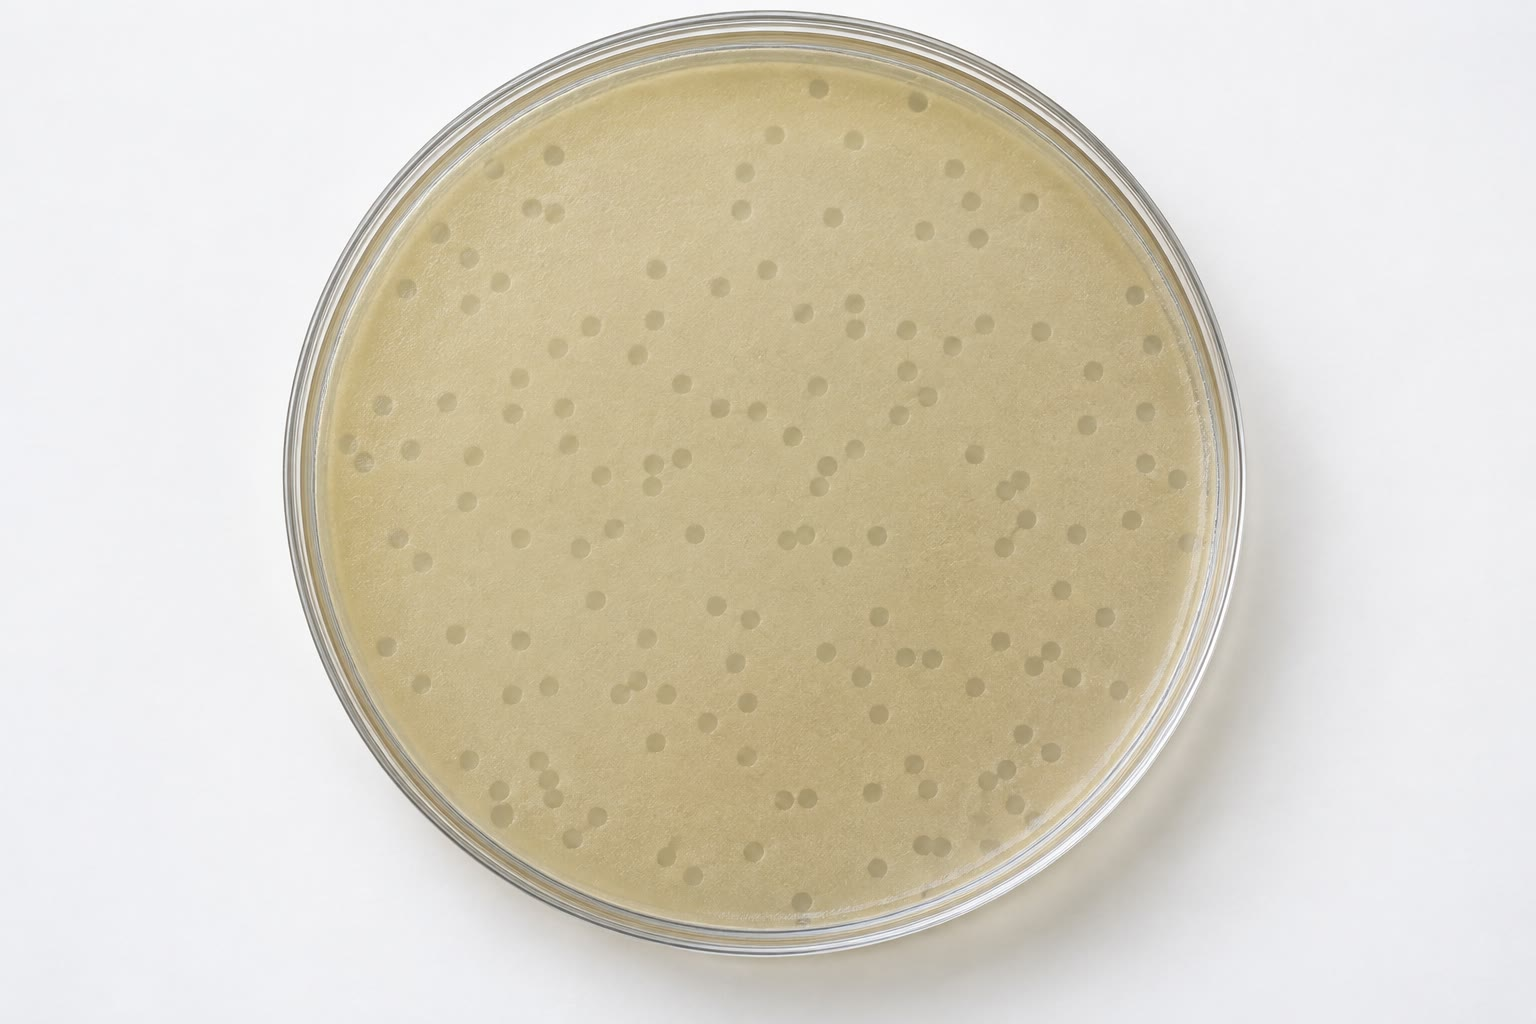
\includegraphics[width=0.46\linewidth]{images/book5/ai/b5-13-plaque-assay.jpg}\hspace{0.04\linewidth}
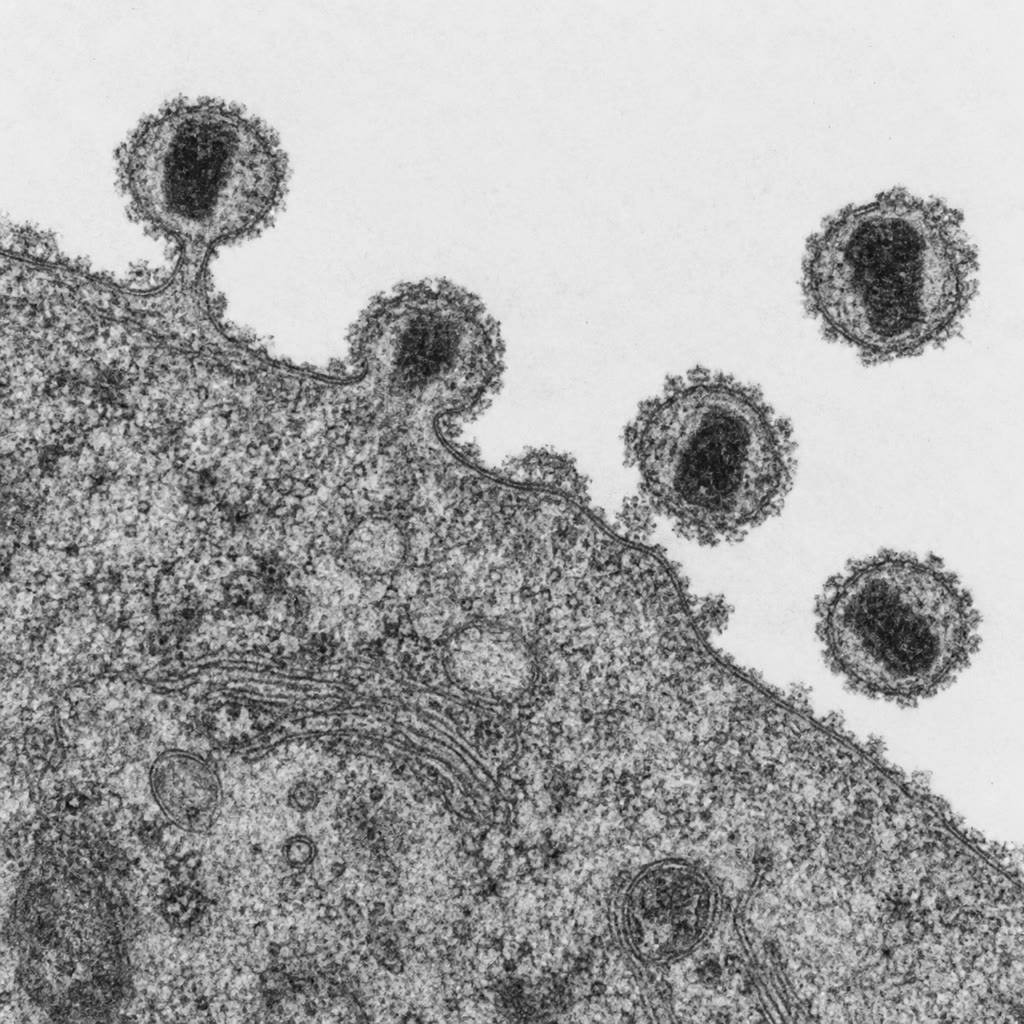
\includegraphics[width=0.36\linewidth]{images/book5/ai/b5-13-hiv-budding.jpg}

{\small Izquierda: placas en un césped bacteriano, cada una una zona
transparente donde la descendencia de un fago ha lisado las células de
alrededor. Derecha: partículas del VIH gemando de un linfocito~T y
tomando su \omterm{def:b3:virology:virus}{envoltura} de la membrana de la célula.}
\end{omfigure}

\begin{theorem}[Dinámica de la infección dentro de un hospedador]\label{thm:b3:virology:dynamics}
\index{número reproductivo básico!dentro del hospedador}\index{carga vírica}\index{dinámica vírica}
Sea $T$ la densidad de células diana susceptibles, $I$ la de células
infectadas y $V$ la de viriones libres. Los viriones infectan dianas a
velocidad $\beta TV$, las células infectadas producen viriones a
velocidad $p$ cada una y mueren a velocidad $\delta$, y los viriones
libres se aclaran a velocidad $c$:
\[
\frac{\mathrm{d}I}{\mathrm{d}t} = \beta TV - \delta I, \qquad
\frac{\mathrm{d}V}{\mathrm{d}t} = pI - cV .
\]
Con $T$ mantenida constante, la infección crece si el \emph{número
reproductivo básico} $R_{0} = \beta Tp/(c\delta)$ supera a $1$, y en el
estado estacionario $V^{*} = p I^{*}/c$, con la producción compensando el
aclaramiento. Si un fármaco detiene todas las infecciones nuevas en
$t = 0$ ($\beta \to 0$), los viriones decaen al principio a la velocidad
de aclaramiento $c$ y después, una vez que el \omterm{def:b3:virology:virus}{virus} libre ha bajado al
nivel que sostienen las células infectadas que quedan, a la velocidad de
muerte $\delta$ de esas células:
\[
V(t) \approx V_{0}\,\frac{c\,e^{-\delta t} - \delta\,e^{-ct}}{c - \delta}
\;\longrightarrow\; V_{0}\,\frac{c}{c-\delta}\,e^{-\delta t}
\quad (t \gg 1/c).
\]
Las dos pendientes de la \omterm{thm:b3:virology:dynamics}{carga vírica} tras el tratamiento miden $c$ y
$\delta$, y $pI^{*} = cV^{*}$ da la producción diaria de viriones antes
del tratamiento.
\end{theorem}
\begin{proof}
Una célula infectada vive de media $1/\delta$ y fabrica $p/\delta$
viriones; cada \omterm{def:b3:virology:virus}{virión} vive $1/c$ e infecta a $\beta T/c$ células en ese
tiempo; el producto es el número de células infectadas al que da lugar
una célula infectada, $R_{0}$. En el estado estacionario
$\mathrm{d}V/\mathrm{d}t = 0$ da $V^{*} = pI^{*}/c$. Tras el tratamiento
$\mathrm{d}I/\mathrm{d}t =
-\delta I$, luego $I = I_{0}e^{-\delta t}$, y $\mathrm{d}V/\mathrm{d}t =
pI_{0}e^{-\delta t} - cV$ es una ecuación lineal cuya solución con
$V(0) = V_{0} = pI_{0}/c$ es la expresión dada (compruébese: en $t = 0$
vale $V_{0}$, y satisface la ecuación término a término). Para $t
\gg 1/c$ el término $e^{-ct}$ ha desaparecido y $V$ sigue a las células
infectadas con pendiente $-\delta$; para $t \ll 1/\delta$ y
$c \gg \delta$ la pendiente inicial es $-c$.
\end{proof}

\begin{example}[El VIH antes y después de las ecuaciones]\label{ex:b3:virology:hiv}
Hasta 1995 los años de \omterm{def:b3:virology:cycle}{latencia} clínica de la infección por el VIH ---
una \omterm{thm:b3:virology:dynamics}{carga vírica} estable de $10^{4}$ a $10^{6}$ copias por mililitro y
una caída lenta de los linfocitos~T --- se leían como un \omterm{def:b3:virology:virus}{virus} quiescente.
Ho, Perelson y colaboradores dieron a unos pacientes un inhibidor de la
proteasa y ajustaron la caída de la \omterm{thm:b3:virology:dynamics}{carga vírica} al teorema: la fase
rápida dio $c \approx \qty{3}{d^{-1}}$ (una semivida del \omterm{def:b3:virology:virus}{virión} de unas
seis horas) y la fase lenta, $\delta \approx
\qty{0.5}{d^{-1}}$ (una célula infectada vive día y medio). Una carga
estable de $10^{5}$ por mililitro en \qty{15}{L} de líquidos corporales,
aclarada a $c$, exige por tanto la producción de unos $10^{10}$ viriones
al día, todos los días, durante años: el período ``latente'' es un estado
estacionario furioso de infección y muerte, con la reserva de linfocitos
T reemplazada a diario hasta que falla. La aritmética de las mutaciones
de la sección siguiente se sigue entonces de inmediato, y con ella la
razón de que los fármacos solos fracasaran y tres no.
\end{example}

\begin{omfigure}
\begin{tikzpicture}
\begin{axis}[
  width=0.7\linewidth, height=5.8cm,
  axis x line=bottom, axis y line=left,
  xmin=0, xmax=14, ymin=10, ymax=2e5, ymode=log,
  xlabel={días desde el inicio del tratamiento}, ylabel={viriones por mL},
  xlabel style={font=\small, at={(axis description cs:0.5,-0.12)}, anchor=north}, ylabel style={font=\small},
  tick label style={font=\small}, xtick={0,2,4,6,8,10,12,14},
  clip=false,
]
\addplot[very thick, omDef, domain=0:14, samples=100] {1e5*(3*exp(-0.5*x) - 0.5*exp(-3*x))/2.5};
\addplot[dashed, omThm, domain=0:1.6, samples=2] {1e5*exp(-3*x)};
\addplot[dashed, omMeth!70!black, domain=1.5:14, samples=2] {1e5*1.2*exp(-0.5*x)};
\node[font=\scriptsize, omThm, anchor=west] at (axis cs:1.8,600) {viriones libres aclarados: pendiente $-c$, semivida \qty{6}{h}};
\node[font=\scriptsize, omMeth!70!black, anchor=south west] at (axis cs:5.5,1.5e4) {células infectadas muriendo: pendiente $-\delta$, semivida \qty{1.4}{d}};
\end{axis}
\end{tikzpicture}

{\small La \omterm{thm:b3:virology:dynamics}{carga vírica} después de que un fármaco detenga las infecciones
nuevas, según el teorema con $c = \qty{3}{d^{-1}}$ y
$\delta = \qty{0.5}{d^{-1}}$: una caída rápida mientras se aclaran los
viriones libres, y después otra más lenta marcada por la muerte de las
células ya infectadas.}
\end{omfigure}

\section{Cómo evolucionan los virus}

\begin{definition}[Mutación, cuasiespecie, deriva y salto]\label{def:b3:virology:evolution}
\index{cuasiespecie}\index{deriva antigénica}\index{salto antigénico}\index{reasociación}
Las polimerasas dependientes de ARN y las transcriptasas inversas no
corrigen pruebas, y los \omterm{def:b3:virology:virus}{virus} de ARN mutan a razón de $10^{-4}$ a
$10^{-6}$ por nucleótido y replicación --- de mil a un millón de veces la
tasa de sus hospedadores ---, de modo que una población de un \omterm{def:b3:virology:virus}{virus} de
ARN es una nube de genomas emparentados, una \emph{cuasiespecie}, en la
que todo mutante puntual está presente en todo momento si la población es
grande. La selección por los anticuerpos impulsa la \emph{deriva
antigénica}: las proteínas de superficie de la gripe acumulan
sustituciones año tras año, y la inmunidad del año pasado protege menos
cada temporada. El \emph{salto antigénico} es un brinco: un genoma
segmentado (la gripe tiene ocho segmentos de ARN) puede
\emph{reasociarse} cuando dos cepas infectan una misma célula, y un
segmento que codifica una hemaglutinina de un \omterm{def:b3:virology:virus}{virus} de ave o de cerdo,
frente a la cual nadie tiene inmunidad, produce una pandemia --- 1918,
1957, 1968, 2009. La recombinación dentro de un genoma hace lo mismo con
los \omterm{def:b3:virology:virus}{virus} no segmentados, y los coronavirus recombinan sin trabas. Casi
todos los \omterm{def:b3:virology:virus}{virus} humanos nuevos son \emph{zoonosis}, que pasan desde un
reservorio animal --- murciélagos para los coronavirus, el Ébola y la
rabia; aves y cerdos para la gripe; primates para el VIH --- y el paso
suele ser cuestión de unas pocas mutaciones en una proteína de unión al
receptor.
\end{definition}

\begin{proposition}[El umbral de error]\label{prop:b3:virology:error-threshold}
\index{umbral de error}\index{corrección de pruebas!vírica}
Un genoma de $L$ nucleótidos copiado con una tasa de error $u$ por
nucleótido se copia sin ningún error con probabilidad
$(1-u)^{L} \approx e^{-uL}$. Para que la secuencia más apta persista en
la población frente a la avalancha de sus mutantes, la fracción de copias
sin error ha de superar aproximadamente el inverso de su ventaja
selectiva $\sigma$: $e^{-uL} \gtrsim
1/\sigma$, es decir, $uL \lesssim \ln\sigma$, un número del orden de uno.
El producto de la tasa de mutación por la longitud del genoma está por
tanto acotado: un \omterm{def:b3:virology:virus}{virus} de ARN con $u = 10^{-4}$ no puede tener un genoma
mucho más largo que $10^{4}$ nucleótidos, que es más o menos lo que
tienen los \omterm{def:b3:virology:virus}{virus} de ARN, y los coronavirus, con sus \qty{30}{kb} los
genomas de ARN más largos conocidos, lo logran solo codificando una
exonucleasa correctora que reduce $u$ diez veces. El umbral es también un
arma: los fármacos que elevan la tasa de error de la polimerasa
(ribavirina, molnupiravir) empujan al \omterm{def:b3:virology:virus}{virus} más allá de él hacia la
\emph{catástrofe de error}, y la \omterm{def:b3:virology:evolution}{cuasiespecie} se desploma.
\end{proposition}
\begin{proof}
Los errores independientes en cada uno de los $L$ sitios dan la
probabilidad de no tener error $(1-u)^{L}$, y $\ln(1-u) \approx -u$ para
$u$ pequeño. El balance poblacional es el argumento habitual de las
\omterm{def:b3:virology:evolution}{cuasiespecies} (Eigen, 1971): la secuencia maestra se repone a velocidad
$\sigma e^{-uL}$ respecto al mutante medio y por lo demás se pierde por
mutación; solo se mantiene si lo primero supera a $1$, de donde la cota.
\end{proof}

\begin{omfigure}
\begin{tikzpicture}[every node/.style={font=\scriptsize}, >=stealth]
  % drift
  \begin{scope}
    \foreach \i in {0,1,2,3} { \draw[thick, omProp, fill=omProp!30] (\i*1.3,0) circle (0.35); \foreach \a in {0,60,...,300} \draw[omProp, thick] (\i*1.3,0) ++(\a:0.35) -- ++(\a:0.14); }
    \foreach \i/\n in {1/1,2/2,3/3} { \foreach \k in {1,...,\n} \fill[omThm] (\i*1.3,0) ++({60*\k+20}:0.5) circle (0.06); }
    \foreach \i in {0,1,2} \draw[->, thick] (\i*1.3+0.5,0) -- (\i*1.3+0.8,0);
    \node[below, align=center] at (1.95,-0.6) {deriva antigénica: las mutaciones puntuales se acumulan\\en las proteínas de superficie, temporada tras temporada};
  \end{scope}
  % shift
  \begin{scope}[xshift=7.0cm]
    \draw[thick, omProp, fill=omProp!30] (0,0.5) circle (0.4); \foreach \y in {-0.2,-0.1,0,0.1,0.2} \draw[omProp!80!black] (-0.25,0.5+\y) -- (0.25,0.5+\y);
    \draw[thick, omMeth!70!black, fill=omMeth!30] (0,-0.7) circle (0.4); \foreach \y in {-0.2,-0.1,0,0.1,0.2} \draw[omMeth!70!black] (-0.25,-0.7+\y) -- (0.25,-0.7+\y);
    \node[left, align=right] at (-0.5,0.5) {cepa humana,\\8 segmentos}; \node[left, align=right] at (-0.5,-0.7) {cepa aviar,\\8 segmentos};
    \draw[->, thick] (0.5,0.4) -- (1.5,0.0); \draw[->, thick] (0.5,-0.6) -- (1.5,-0.2);
    \draw[thick, omDef, fill=omDef!10] (2.4,-0.1) ellipse (0.9 and 0.7); \node[below] at (2.4,-0.85) {una célula (un cerdo)};
    \draw[->, thick] (3.4,-0.1) -- (4.3,-0.1);
    \draw[thick, omProp, fill=omProp!30] (4.9,-0.1) circle (0.4); \foreach \y in {-0.2,-0.1,0.1,0.2} \draw[omProp!80!black] (4.65,-0.1+\y) -- (5.15,-0.1+\y); \draw[omMeth!70!black, very thick] (4.65,-0.1) -- (5.15,-0.1);
    \node[right, align=left] at (5.2,-0.1) {reasociante:\\hemaglutinina\\aviar en un\\virus humano};
    \node[below, align=center] at (2.4,-1.5) {salto antigénico: se intercambian segmentos enteros;\\nadie es inmune --- una pandemia};
  \end{scope}
\end{tikzpicture}

{\small Dos maneras que tiene un \omterm{def:b3:virology:virus}{virus} de la gripe de escapar a la
inmunidad. La deriva: las mutaciones de las espículas se acumulan poco a
poco. El salto: dos cepas en una misma célula intercambian segmentos
enteros del genoma, y aparece de golpe una proteína de espícula nueva
para el ser humano.}
\end{omfigure}

\begin{example}[Por qué el VIH necesitó tres fármacos]\label{ex:b3:virology:three-drugs}
La transcriptasa inversa del VIH se equivoca aproximadamente una vez de
cada $10^{5}$ nucleótidos, de modo que cada genoma de \qty{9700}{nt}
copiado lleva unas $0.1$ mutaciones, y $10^{10}$ genomas nuevos al día
llevan entre todos $10^{9}$ mutaciones: cada una de las
$3\times 9700 \approx \num{30000}$ mutaciones puntuales posibles surge
muchas veces cada día, antes de que se dé ningún fármaco. Un fármaco al
que derrota una sola mutación --- como una sola mutación derrota a casi
todos los inhibidores de la transcriptasa inversa y de la proteasa ---
queda por tanto derrotado en semanas, que es lo que le ocurrió a la AZT
en 1987. Dos mutaciones independientes surgen juntas a $10^{-10}$ por
genoma, alrededor de una vez al día; tres, a $10^{-15}$, una vez cada mil
días --- y un paciente con tres fármacos cuya carga ha caído mil veces
produce $10^{7}$ genomas al día, de modo que el triple mutante no aparece
nunca. Eso, junto con la demostración del teorema de que el \omterm{def:b3:virology:virus}{virus} se
replicaba a toda velocidad, hizo de la \omterm{thm:b3:cancer-biology:goldie-coldman}{terapia combinada}, desde 1996, el
tratamiento que convirtió el sida en una enfermedad crónica.
\end{example}

\section{Hospedadores, defensas y fármacos}

\begin{proposition}[Patogenia y defensa]\label{prop:b3:virology:pathogenesis}
\index{efecto citopático}\index{interferón}\index{restricción!de fagos}
Un \omterm{def:b3:virology:virus}{virus} daña lisando células (la polio destruye motoneuronas, el VIH
mata linfocitos~T), haciendo que las células fabriquen productos tóxicos,
transformándolas (\cref{ch:b3:cancer-biology}) y a menudo, sobre todo, a
través de la propia respuesta del hospedador: la fiebre, el daño tisular
y, en el peor de los casos, la tormenta de citocinas de la reacción
inmunitaria a la gripe o a los coronavirus del SARS. El hospedador
responde con defensas innatas que reconocen las firmas de la replicación
vírica --- ARN de doble hebra, ARN sin caperuza, ADN en el citosol --- y
responden con \emph{interferón}, que pone a todas las células vecinas en
un estado \omterm{def:b3:virology:drugs}{antivírico} (\cref{ch:b3:innate-immunity}); con linfocitos
citolíticos naturales que destruyen las células que han escondido su MHC;
con anticuerpos que neutralizan viriones y linfocitos~T citotóxicos que
matan a las células infectadas antes de que liberen descendencia
(\cref{ch:b3:adaptive-immunity}); y, en las bacterias, con \omterm{def:b3:genetic-engineering:tools}{enzimas de
restricción} que cortan el ADN ajeno y con la memoria \omterm{def:b3:genetic-engineering:crispr}{CRISPR} del
\cref{ch:b3:genetic-engineering}. Los \omterm{def:b3:virology:virus}{virus} contestan: casi todo \omterm{def:b3:virology:virus}{virus}
grande codifica proteínas que bloquean el interferón, esconden el MHC,
imitan citocinas o inhiben la \omterm{def:b3:cell-cycle-apoptosis:apoptosis}{apoptosis}, y la carrera de armamentos está
escrita en los dos genomas.
\end{proposition}

\begin{definition}[Antivíricos y vacunas]\label{def:b3:virology:drugs}
\index{antivírico}\index{análogo de nucleósido}\index{inhibidor de proteasa}\index{vacuna}\index{vacuna de ARNm}
Los antivíricos atacan las enzimas víricas o los pasos que una célula
hospedadora no lleva a cabo. Los \emph{análogos de nucleósido} son
terminadores de cadena: el aciclovir solo lo fosforila la
timidina-quinasa del herpesvirus y bloquea después la ADN-polimerasa
vírica, de modo que actúa solo en las células infectadas; la AZT, el
tenofovir y la lamivudina detienen la transcriptasa inversa; el
remdesivir y el molnupiravir actúan sobre la polimerasa del coronavirus,
el segundo por mutagénesis. Los \emph{inhibidores de proteasa} bloquean
el corte de las poliproteínas víricas (el VIH, la hepatitis C, el
nirmatrelvir del SARS-CoV-2). Los inhibidores de la integrasa impiden que
se forme el provirus del VIH; los de la neuraminidasa impiden que los
viriones de la gripe se desprendan de la célula de la que geman; y los
inhibidores de entrada bloquean un receptor. El \omterm{def:b3:virology:virus}{virus} de la hepatitis C
se cura hoy en doce semanas con combinaciones de fármacos de acción
directa, la primera infección vírica crónica curada por quimioterapia.
Las \emph{vacunas} presentan los antígenos del \omterm{def:b3:virology:virus}{virus} sin su enfermedad:
un \omterm{def:b3:virology:virus}{virus} vivo atenuado (sarampión, polio por vía oral, fiebre amarilla),
un \omterm{def:b3:virology:virus}{virus} inactivado (polio inyectada, gripe), una subunidad (el antígeno
de superficie de la hepatitis B fabricado en levadura, la proteína de la
\omterm{def:b3:virology:virus}{cápside} del papilomavirus), un vector vírico inocuo que lleva un gen de
la diana o, desde 2020, \emph{ARN mensajero} que codifica el antígeno,
entregado en nanopartículas lipídicas, que las propias células de quien
lo recibe traducen. La inmunología de por qué funcionan, y de cuántas
personas han de vacunarse para proteger al resto, es asunto del
\cref{ch:b3:adaptive-immunity}.
\end{definition}

\begin{remark}[Los virus en la economía de la vida]\label{rem:b3:virology:economy}
Los \omterm{def:b3:virology:virus}{virus} que dañan al ser humano son un error de redondeo en la
población vírica del mundo, que en su mayor parte infecta a bacterias y
arqueas. Los fagos matan cada día de una quinta a una tercera parte de
las bacterias del océano y devuelven su contenido a la reserva disuelta
--- la \emph{derivación vírica} del ciclo del carbono del volumen de
segundo año. Mueven genes entre bacterias (\cref{ch:b3:bacteriology}), y
sus toxinas son las toxinas de la difteria, el cólera y las peores
\emph{E.~coli}. El ocho por ciento del genoma humano son los restos de
retrovirus antiguos (\cref{ch:b3:genomics}), y uno de sus genes de
\omterm{def:b3:virology:virus}{envoltura} fusiona hoy las células de la placenta. Los \omterm{def:b3:virology:virus}{virus} son el mayor
reservorio de novedad genética del planeta, y la frontera de lo que
cuenta como vivo pasa por ellos.
\end{remark}

\section{Ejercicios}

\begin{exercise}[$\star$]\label{exo:b3:virology:1}
Sitúense la polio, la gripe, el VIH, el herpes simple, la hepatitis B y
el rotavirus en sus clases de Baltimore y dígase qué enzima ha de traer o
fabricar cada uno que la célula no tiene.
\end{exercise}

\begin{exercise}[$\star$]\label{exo:b3:virology:2}
¿Qué mostró el experimento de Hershey y Chase, y qué se habría encontrado
si la proteína llevara las instrucciones?
\end{exercise}

\begin{exercise}[$\star$]\label{exo:b3:virology:3}
Una reserva de fago diluida $10^{-7}$ da $84$ placas a partir de
\qty{0.1}{mL}. ¿Cuál es el título? ¿Por qué puede el microscopio
electrónico contar diez veces más partículas?
\end{exercise}

\begin{exercise}[$\star$]\label{exo:b3:virology:4}
Enumérense las seis etapas de un ciclo de replicación y, para cada una,
nómbrese un \omterm{def:b3:virology:drugs}{antivírico} o una defensa del hospedador que actúe sobre ella.
\end{exercise}

\begin{exercise}[$\star\star$]\label{exo:b3:virology:5}
Con la \cref{prop:b3:virology:economy}, calcúlese el ácido nucleico
necesario para codificar la \omterm{def:b3:virology:virus}{cápside} de un \omterm{def:b3:virology:virus}{virus} hecho de $180$ copias de
una proteína de \qty{30}{kDa}, y compárese con el genoma de \qty{4.5}{kb}
que podría tener un \omterm{def:b3:virology:virus}{virus} así. ¿Qué fracción del genoma es el gen de la
\omterm{def:b3:virology:virus}{cápside}?
\end{exercise}

\begin{exercise}[$\star\star$]\label{exo:b3:virology:6}
Con $c = \qty{3}{d^{-1}}$, $\delta = \qty{0.5}{d^{-1}}$ y $V_{0} =
10^{5}$ por mL, calcúlese $V$ con el teorema en $t = 0.5$, $2$ y $10$
días. ¿Cuánto tarda la carga en bajar de $50$ por mL, el límite de
detección?
\end{exercise}

\begin{exercise}[$\star\star$]\label{exo:b3:virology:7}
Un \omterm{def:b3:virology:virus}{virus} de ARN tiene $u = 3\times 10^{-5}$ y $L = \qty{12}{kb}$. ¿Qué
fracción de sus genomas descendientes no lleva ninguna mutación? ¿Qué le
ocurre a esa fracción si un fármaco mutagénico triplica $u$? Explíquese
por qué los coronavirus necesitaron una enzima correctora.
\end{exercise}

\begin{exercise}[$\star\star$]\label{exo:b3:virology:8}
Explíquense la deriva y el \omterm{def:b3:virology:evolution}{salto antigénicos} en la gripe, y por qué toda
cepa pandémica ha llevado hasta ahora una hemaglutinina nueva.
\end{exercise}

\begin{exercise}[$\star\star$]\label{exo:b3:virology:9}
El aciclovir es un análogo de la guanosina que ha de fosforilarse para
actuar. Explíquese por qué daña a las células infectadas por el herpes y
no a las demás, y predíganse las mutaciones de resistencia.
\end{exercise}

\begin{exercise}[$\star\star\star$]\label{exo:b3:virology:10}
Dedúzcase $R_{0} = \beta Tp/(c\delta)$ a partir de las dos ecuaciones del
teorema, hallando la condición para que una infección pequeña ($I$ y $V$
cerca de cero, $T$ constante) crezca, e interprétese cada factor.
\end{exercise}

\begin{exercise}[$\star\star\star$]\label{exo:b3:virology:11}
Un paciente con tratamiento eficaz alberga aún $10^{6}$ linfocitos~T en
reposo infectados de forma latente, cuyo provirus está silencioso, con
una semivida de $44$ meses. ¿Cuánto tendría que durar el tratamiento para
que el reservorio bajara de una célula? ¿Por qué hace esto que el VIH sea
incurable con fármacos que bloquean la replicación, y qué exigiría una
cura?
\end{exercise}

\begin{exercise}[$\star\star\star$]\label{exo:b3:virology:12}
Explíquese el argumento del \cref{ex:b3:virology:three-drugs} con números
propios para un \omterm{def:b3:virology:virus}{virus} de \qty{30}{kb} con $u = 10^{-6}$ que produce
$10^{9}$ genomas al día. ¿Cuántos fármacos se combinarían, y por qué unos
fármacos contra dos sitios de la misma enzima podrían no contar como dos?
\end{exercise}

\section{Problema: un virus en un paciente}

\begin{problem}[{Problema de fin de semana --- una infección por el VIH
contada virión a virión, su dinámica ajustada a una curva de tratamiento,
sus mutaciones sumadas frente a los fármacos y su reservorio
cronometrado, hasta llegar a la producción diaria de viriones, al día en
que la carga se vuelve indetectable y a la probabilidad de que exista un
triple mutante}]
\label{pb:b3:virology:1}
Datos: \omterm{thm:b3:virology:dynamics}{carga vírica} $V^{*} = 2\times 10^{5}$ por mL en \qty{15}{L} de
líquidos corporales; $c = \qty{3}{d^{-1}}$, $\delta = \qty{0.5}{d^{-1}}$;
cada célula infectada fabrica $p = 500$ viriones al día; genoma de
\qty{9700}{nt}, $u = 10^{-5}$ por nucleótido y replicación; mutaciones
únicas confieren resistencia a cada uno de tres fármacos; con triple
terapia la producción cae a $10^{7}$ genomas al día; reservorio latente
de $10^{6}$ células, con semivida de $44$ meses; un \omterm{def:b3:virology:virus}{virión} es una esfera
de \qty{120}{nm} que contiene dos hebras de ARN de \qty{9700}{nt} y unas
\num{2000} moléculas de proteína de \qty{25}{kDa}.

\medskip
\noindent\textbf{Parte I --- Contar.}
\begin{enumerate}
  \item ¿Cuántos viriones hay en el cuerpo en el estado estacionario?
  \item ¿Cuántos se aclaran al día y, por tanto, cuántos se producen al
        día?
  \item ¿Cuántas células infectadas los producen, y cuántas mueren al
        día?
  \item ¿Cuál es la masa de un \omterm{def:b3:virology:virus}{virión} (ARN a \qty{330}{Da} por nucleótido
        más la proteína), y la masa total de viriones del cuerpo?
        Compárese con un grano de arena (\qty{1}{mg}).
  \item El cuerpo tiene $10^{12}$ linfocitos~T CD4 y repone los
        infectados. ¿Qué fracción de la reserva está infectada en cada
        momento, y cómo mata a la reserva en diez años una fracción tan
        pequeña?
  \item Si cada célula infectada muere por \omterm{def:b3:cell-cycle-apoptosis:apoptosis}{apoptosis} y es engullida en
        menos de una hora (\cref{ch:b3:cell-cycle-apoptosis}), ¿cuántas
        se están eliminando en cada momento?
\end{enumerate}

\medskip
\noindent\textbf{Parte II --- El tratamiento.}
\begin{enumerate}[resume]
  \item El tratamiento detiene las infecciones nuevas en $t = 0$.
        Calcúlese $V$ con el teorema en $t =
        1$, $3$, $7$ y $14$ días.
  \item ¿Qué día baja la carga del límite de detección de $50$ por mL?
  \item A partir de las dos pendientes, ¿cómo estimaría un clínico $c$ y
        $\delta$ con medidas de los días $0$--$1$ y $3$--$10$?
  \item Tras las dos fases la carga se aplana en unas pocas copias por mL
        y se queda ahí durante años. ¿Qué compartimento del modelo falta,
        y cuál es su velocidad de decaimiento?
  \item Calcúlense la semivida de un \omterm{def:b3:virology:virus}{virión} libre y la de una célula
        infectada.
  \item Explíquese por qué la meseta anterior al tratamiento se
        interpretó mal como \omterm{def:b3:virology:cycle}{latencia}, y qué mostraron en cambio las
        ecuaciones.
\end{enumerate}

\medskip
\noindent\textbf{Parte III --- La mutación.}
\begin{enumerate}[resume]
  \item Mutaciones por genoma y replicación, y mutaciones producidas al
        día en el paciente sin tratar.
  \item ¿Cuántas mutaciones puntuales distintas son posibles en el
        genoma? ¿Cuántas veces al día surge cada una?
  \item Velocidad por genoma de un doble mutante concreto y de un triple
        mutante concreto; ¿cuántos de cada uno surgen al día sin
        tratamiento?
  \item Con triple terapia y $10^{7}$ genomas al día, ¿triples mutantes
        esperados al año?
  \item El paciente se salta dosis, de modo que el nivel de un fármaco
        cae a cero durante una semana mientras los otros dos se
        mantienen. ¿Qué mutantes pueden seleccionarse ahora, y cuál es el
        número esperado de los dobles mutantes pertinentes producidos en
        esa semana a $10^{7}$ genomas al día?
  \item ¿Por qué la resistencia a un \omterm{def:b3:virology:drugs}{análogo de nucleósido} confiere a
        menudo resistencia a otro, y cómo cambia eso el recuento de
        fármacos ``independientes''?
\end{enumerate}

\medskip
\noindent\textbf{Parte IV --- El reservorio y la cura.}
\begin{enumerate}[resume]
  \item Con una semivida de $44$ meses, ¿cuánto tardan las $10^{6}$
        células latentes en bajar a una? ¿Y a $10^{4}$?
  \item Si se interrumpe el tratamiento, basta con que se reactive una
        célula latente para reiniciar la infección. ¿Cuánto tarda la
        carga en volver a $10^{5}$ por mL tras la interrupción, si crece
        con $R_{0} = 8$ por generación de $2$ días a partir de un solo
        \omterm{def:b3:virology:virus}{virión}?
  \item Propónganse dos estrategias de cura que se sigan del modelo, y
        enúnciese el obstáculo de cada una.
  \item El $R_{0}$ del teorema es dentro de un hospedador. Un $R_{0}$
        poblacional del VIH entre personas es de unos $3$ a $5$. ¿Qué
        fracción de las transmisiones hay que evitar para acabar con la
        epidemia ($1 - 1/R_{0}$)?
  \item El tratamiento baja la transmisibilidad de un paciente
        prácticamente a cero. Explíquese cómo se sigue el ``tratamiento
        como prevención'' del teorema de dentro del hospedador.
  \item Una \omterm{def:b3:virology:drugs}{vacuna} de eficacia $E$ (la fracción de vacunados protegidos)
        administrada a una fracción $f$ de la población protege a $Ef$ de
        ella. ¿Qué cobertura $f$ hace falta para llegar al umbral de la
        pregunta anterior con $E = 0.7$? ¿Y con $E = 0.9$? ¿Qué
        significa la primera respuesta?
  \item Resúmase: los viriones producidos al día (pregunta~2), el día en
        que la carga se vuelve indetectable (pregunta~8) y el número
        esperado de triples mutantes al año con tratamiento
        (pregunta~16).
\end{enumerate}
\end{problem}
